%seed - 98237187966

\documentclass{article}

\usepackage[margin=0.75in,left=0.5in,right=0.5in]{geometry}
\usepackage{mymath}
\usepackage{pytex}

\begin{document}

\begin{enumerate}

        
  \item
    File: antiderivative-indefinite-simple-mixed-1.tex\\
    % This gives students a function to find a basic antiderivative
% using basic rules.


Find the antiderivative of the function $\displaystyle f(x)= - 5 \sqrt[4]{x} - 9 x^{2} - 8 e^{x} + 4 \sec^{2}{\left(x \right)} - 3 - \frac{6}{x}$

  \item
    File: area-exact\_geometry-1.tex\\
    %
Calculate the exact area under the curve of $f(x)=4 - \left|{x}\right|$ on $[-4,4]$. 
  \item
    File: area\_rectangle\_approximation-graph\_provided-1.tex\\
    Approximate the area of the shaded region using 4 left endpoint rectangles.

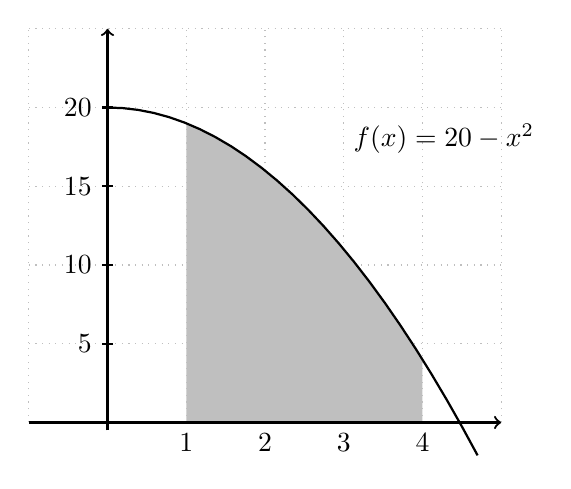
\begin{tikzpicture}[yscale=.2]
  \fill [lightgray, domain=1:4] (1,0) -- plot ({\x},{20-(\x)^2}) -- (4,0) -- cycle;
  % axes
  \draw [dotted, lightgray, ystep=5] (-1,0) grid (5,25);
  \draw [thick, ->] (-1,0) -- (5,0);
  \draw [thick, ->] (0,-0.5) -- (0,25);
  % axis labels
  \foreach \x in {1,2,3,4} {
    \draw [thick] (\x, 2pt) -- (\x, -2pt) node [below] {$\x$};
  };
  \foreach \y in {5, 10, 15, 20} {
    \draw [thick] (2pt, \y) -- (-2pt, \y) node [left] {$\y$};
  };
  %
  \draw [thick, domain=0:4.7] plot ({\x},{20-(\x)^2});
  \draw (3,18) node[right] {$f(x)=20-x^2$};
  
\end{tikzpicture}

  \item
    File: area\_rectangle\_approximation-graph\_provided-2.tex\\
    Approximate the area of the shaded region using 4 left endpoint rectangles.

\begin{tikzpicture}[yscale=2]
  \fill [lightgray, domain=1:4] (1,0) -- plot (\x,1/\x) -- (4,0) -- cycle;
  % axes
  \draw [dotted, lightgray] (-1,-0.5) grid (5,2);
  \draw [thick, ->] (-1,0) -- (5,0);
  \draw [thick, ->] (0,-0.5) -- (0,2);
  % axis labels
  \foreach \x in {1,2,3,4} {
    \draw [thick] (\x, 2pt) -- (\x, -2pt) node [below] {$\x$};
  };
  \foreach \y in {1} {
    \draw [thick] (2pt, \y) -- (-2pt, \y) node [left] {$\y$};
  };
  %
  \draw [thick, domain=0.5:5] plot (\x,1/\x);
  \draw (2,1) node[right] {$f(x)=\dfrac{1}{x}$};
  
\end{tikzpicture}

  \item
    File: area\_rectangle\_approximation-graph\_provided-3.tex\\
    Approximate the area of the shaded region using 4 left endpoint rectangles.

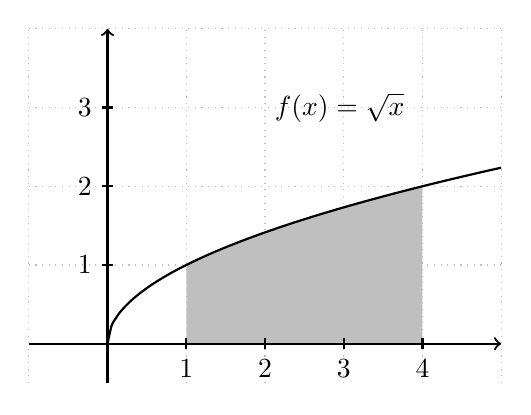
\begin{tikzpicture}[yscale=1]
  \fill [lightgray, domain=1:4] (1,0) -- plot ({\x},{\x^(1/2)}) -- (4,0) -- cycle;
  % axes
  \draw [dotted, lightgray] (-1,-0.5) grid (5,4);
  \draw [thick, ->] (-1,0) -- (5,0);
  \draw [thick, ->] (0,-0.5) -- (0,4);
  % axis labels
  \foreach \x in {1,2,3,4} {
    \draw [thick] (\x, 2pt) -- (\x, -2pt) node [below] {$\x$};
  };
  \foreach \y in {1,2,3} {
    \draw [thick] (2pt, \y) -- (-2pt, \y) node [left] {$\y$};
  };
  %
  \draw [thick, domain=0:5, smooth, samples=100] plot ({\x},{\x^(1/2)});
  \draw (2,3) node[right] {$f(x)=\sqrt{x}$};
  
\end{tikzpicture}

  \item
    File: concavity-increase-graphical-1.tex\\
    % This produces a function that requests students to find the global
% extrema on a particular interval. This uses the same curve each time
% but uses left and right shifts to make it look different each time


Use the graph below to answer the questions that follow. Some important $x$ and $y$ values occur at non-integer values, please just estimate them to the nearest half of a unit. \\[4mm]
\begin{minipage}{0.45\textwidth}
  \begin{tikzpicture}[scale=0.65]
    % axes
    \draw [dotted, lightgray] (-5,-5) grid (5,5);
    \draw [thick, <->] (-6,0) -- (6,0);
    \draw [thick, <->] (0,-6) -- (0,6);
    % axis labels
    \foreach \x in {-5,-4,-3,-2,-1,1,2,3,4,5} {
      \draw [thick] (\x, 5pt) -- (\x, -5pt) node [below] {$\scriptstyle \x$};
      \draw [thick] (5pt, \x) -- (-5pt, \x) node [left] {$\scriptstyle \x$};
    }
    % function
    \draw [<->, myblue, very thick, domain=-4.4:3.45,smooth] plot ({\x},{1.0*0.068*((\x)+3)^2*(\x)*((\x)-3)}); 
  \end{tikzpicture}
\end{minipage}
%
\begin{minipage}{0.45\textwidth}
  \raggedright
  \begin{enumerate}[a.]
    \item Determine the intervals for which the function is:
    \begin{itemize}[label={},itemsep=5mm]
      \item Increasing: \hrulefill
      \item Decreasing: \hrulefill
      \item Concave Up: \hrulefill
      \item Concave Down: \hrulefill
    \end{itemize}
    \item Identify any inflection points.
  \end{enumerate}
  \vspace{10mm}
\end{minipage}

  \item
    File: continuity-graphical-1.tex\\
    % This produces a graph that has three different types of discontinuities,
% a hole, a vertical asymptote, and a jump. The student is then asked
% multiple questions involving limits and function values.


The graph below depicts a function $f(x)$. Use it to identify any discontinuities and label them as either removable or non-removable. \\

\begin{tikzpicture}[scale=0.75]
    \draw [->] (-5.5,0) -- (5.5,0) node[right] {$x$};
    \draw [->] (0,-5.5) -- (0,5.5) node[right] {$y$};
    \draw [dotted] (-5,-5) grid (5,5);
    
    \foreach \x in {-5,-4,-3,-2,-1,1,2,3,4,5} {
      \draw (\x,0) to (\x,-3pt);
      \draw (\x,-3pt) node[below] {\scriptsize \x};
    }
    
    \foreach \y in {-5,-4,-3,-2,-1,1,2,3,4,5} {
      \draw (0,\y) to (-3pt,\y);
      \draw (-3pt,\y) node[left] {\scriptsize \y};
    }
    
    %asymptote
    \draw [<->, myblue, very thick] (-5.5,-2.1) to[out=20,in=260] (-3.1, 5);
    \draw [<-, myblue, very thick] (-2.9,-5) to[out=90,in=135] (-1,1);
    \draw [myblue, very thick, dashed] (-3,-5) -- (-3,5);
    \draw [myblue, very thick, fill=white] (-1,1) circle (3pt);
    %segment 1
    \draw [myblue, fill=myblue] (-1,-2) circle (3pt);
    \draw [very thick, myblue] (-1,-2) to (1, 3);
    %segment 2
    \draw [myblue, very thick, fill=white] (1,3) circle (3pt);
    \draw [->, myblue, very thick] (1,3) to[out=0,in=180] (5,-2);
    
\end{tikzpicture}

  \item
    File: derivative-chain-radical-1.tex\\
    % This gives students a function to differentiate that requires the use
% of the the chain rule within a radical expression


Differentiate: $y = \sqrt[3]{x^{5} - 3 x}$

  \item
    File: derivative-implicit-1.tex\\
    % This produces a polynomial relation in implicit form to
% differentiate.
%
% This particular questin will require the product rule


Differentiate: $- 6 x^{4} - 5 x^{3} y^{2} + 5 y^{5}=-15$

  \item
    File: derivative-logarithm-quotient-1.tex\\
    % This produces a function to differentiation that contains a logarithm
% of a quotient that can be more easily evaluated if the student first
% uses rules of logarithms


Differentiate: $\displaystyle f(x)=\log{\left(\frac{x^{3} - 5 x}{- 3 x^{4} + x^{3}} \right)}$

  \item
    File: derivative-powerrule-1.tex\\
    % This gives students a function to differentiate using the
% power rule in different ways. 


Differentiate: $y = \displaystyle \frac{1}{5} x^{5} + 2 \sqrt[5]{x} - \frac{-11}{x^{1/3}} + 12$

  \item
    File: derivative-product-chain-1.tex\\
    % This gives students a function to differentiate that requires the use
% of the product rule and the chain rule


Differentiate: $y = 5 x^{4} \sin{\left(x^{2} - 4 x \right)}$

  \item
    File: derivative-quotient-basic-1.tex\\
    % This gives students a function to differentiate using the
% power rule in different ways. 


Differentiate: $f(x) = \dfrac{2 x^{2} - 10}{2 e^{x}}$

  \item
    File: derivative-sketch-1.tex\\
    % This will create a graph that a student needs to sketch the
% graph of it's derivative.


Sketch a possible graph of the derivative of the function shown. 

\begin{tikzpicture}[scale=1]
  \draw [dotted, black] (-5,-5) grid (5,5);
  \draw [->] (-5,0) -- (5,0) node[right] {$x$};
  \draw [->] (0,-5) -- (0,5) node[above] {$y$};
  \foreach \x in {-5,-4,-3,-2,-1,1,2,3,4,5} {
    \draw (\x,0) to (\x,-3pt);
    \draw (\x,-3pt) node[below] {\scriptsize \x};
  }
  \foreach \y in {-5,-4,-3,-2,-1,1,2,3,4,5} {
    \draw (0,\y) to (-3pt,\y);
    \draw (-3pt,\y) node[left] {\scriptsize \y};
  }
  %parabola
  \draw [very thick, myblue, domain=-1:2,smooth] plot (\x, {-(\x)^2+3});
  \draw [myblue, fill=white] (-1,2) circle (3pt);
  \draw [myblue, fill=myblue] (2,-1) circle (3pt);
  %horizontal line
  \draw [<-,very thick, myblue] (-5,4) -- (-1,4);
  \draw [myblue, fill=myblue] (-1,4) circle (3pt);
  %oblique line
  \draw [->, very thick, myblue] (2,1) -- (5,-2);
  \draw [myblue, fill=white] (2,1) circle (3pt);
\end{tikzpicture}

  \item
    File: extrema-global-polynomial-1.tex\\
    % This produces a function that requests students to find the global
% extrema on a particular interval. This uses the same curve each time
% but uses left and right shifts to make it look different each time


Find the global extrema for the function $ f(x)=\left(x^{2} - 4 x\right)^{2} $ on the closed interval $[1, 5]$.

\begin{enumerate}[a.]
  \item Global Minimum: \rule{6cm}{0.15mm} \\[8mm]
  \item Global Maximum: \rule{6cm}{0.15mm} \\[8mm]
\end{enumerate}  

  \item
    File: extrema-graphical-global-local-1.tex\\
    % This produces a function that requests students to find the global
% extrema on a particular interval. This uses the same curve each time
% but uses left and right shifts to make it look different each time


Use the graph below to answer the questions that follow. Some important $x$ and $y$ values occur at non-integers, please just estimate them to the nearest half of a unit. \\[4mm]
\begin{minipage}{0.45\textwidth}
  \begin{tikzpicture}[scale=0.7]
    % axes
    \draw [dotted, lightgray] (-5,-5) grid (5,5);
    \draw [thick, <->] (-6,0) -- (6,0);
    \draw [thick, <->] (0,-6) -- (0,6);
    % axis labels
    \foreach \x in {-5,-4,-3,-2,-1,1,2,3,4,5} {
      \draw [thick] (\x, 5pt) -- (\x, -5pt) node [below] {$\scriptstyle \x$};
      \draw [thick] (5pt, \x) -- (-5pt, \x) node [left] {$\scriptstyle \x$};
    }
    % function
    \draw [<->, myblue, very thick] plot[smooth] coordinates {(-5,-5.0) (-3,3.0) (0,-1.0) (2,1.0) (5, -5.0)};
  \end{tikzpicture}
\end{minipage}
%
\begin{minipage}{0.45\textwidth}
  \begin{enumerate}[a.]
    \item Identify any global extrema: \\[3cm]
    \item Identify any local extrema: \\[2cm]
  \end{enumerate}
\end{minipage}

  \item
    File: first\_derivative\_test-extrema-intervals-1.tex\\
    % This will create a function that students are asked to determine
% where the function is increasing or decreasing, and identify the
% locations of any local extrema. For time-savings, the first and
% second derivatives are already provided.


Given the function $ \displaystyle f(x) = \frac{x^{2}}{4 \left(x + 3\right)} $, identify the location of any local extrema (only $x$-values), and the intervals for which the function is increasing, or decreasing. \\[4mm]

For simplicity, the first and second derivatives are:

$ \displaystyle f'(x)=\frac{x \left(x + 6\right)}{4 \left(x + 3\right)^{2}} $, and $ \displaystyle f''(x)=\frac{9}{2 \left(x + 3\right)^{3}} $

\vspace{6cm}

\begin{tasks}[label={},after-item-skip=6mm](2)
  \task Increasing: \hrulefill 
  \task Decreasing: \hrulefill 
  \task Local Minima: \hrulefill 
  \task Local Maxima: \hrulefill 
\end{tasks}

  \item
    File: first\_derivative\_test-no\_function-label\_extrema-1.tex\\
    % This gives students a set of critical values of an unknown
% function placed along a number line and whether the derivative
% of the function is positive or negative. The students are then
% asked to determine whether the critical values are local
% minimums, maximums or neither.


The following intervals indicate where the first derivative of a function is either positive or negative. Each value on the number line is a critical value of the function. Label each critical number that appears on the number line as a local minimum, local maximum, or neither.

\begin{center}
  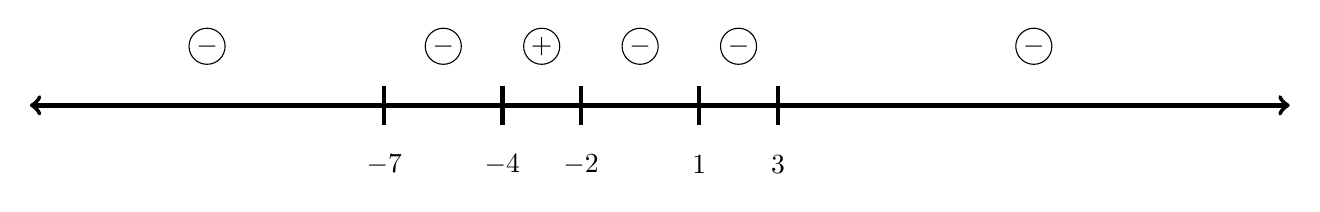
\begin{tikzpicture}[scale=0.5]
    
    \draw [<->, ultra thick] (-16,0) -- (16,0);
    \foreach \x in {-7,-4,-2,1,3} {
      \draw [ultra thick] (\x,-0.5) -- (\x,0.5);
      \draw (\x, -1.5) node {$\x$};
    }

    \node[draw, circle, inner sep=1pt] at (-11.5, 1.5) {$-$};
    \node[draw, circle, inner sep=1pt] at (-5.5, 1.5) {$-$};
    \node[draw, circle, inner sep=1pt] at (-3.0, 1.5) {$+$};
    \node[draw, circle, inner sep=1pt] at (-0.5, 1.5) {$-$};
    \node[draw, circle, inner sep=1pt] at (2.0, 1.5) {$-$};
    \node[draw, circle, inner sep=1pt] at (9.5, 1.5) {$-$};

  \end{tikzpicture}
\end{center}

  \item
    File: integral-definite-geometry-1.tex\\
    % Gives the student a function that they can use a formula
% from geometry to calculate the value of the definite integral


Calculate the exact area under the curve of $f(x)=\sqrt{16 - x^{2}}$ on $[-4,4]$.
  \item
    File: integral-definite-polynomial-1.tex\\
    $ \dint_{5}^{7} x^{2} + 4 x \dx $
  \item
    File: integral-definite-properties-1.tex\\
    % Gives the student a definite integral to evaluate using only
% properties of definite integrals as no functions are provided.
%
%
Evaluate the definite integral $\dint_{4}^{15} 5 f{\left(x \right)} + g{\left(x \right)} + 3 \dx$ given that: \\ $\dint_{9}^{15} f(x) \dx = 1$, $\dint_{4}^{9} f(x) \dx = 4$, and $\dint_{15}^{4} g(x) \dx = 3$.

  \item
    File: integral-definite-properties-2.tex\\
    %
Use the properties of definite integrals to combine the following statements into a single integral. You may find it helpful to draw out a sketch of what the region could look like.
$$ \dint_{-12}^{2} f(x) \dx + \dint_{2}^{8} f(x) \dx - \dint_{-12}^{-3} f(x) \dx $$

  \item
    File: integral-definite-substitution-power\_rule-1.tex\\
    %
Evaluate the definite integral: $\dint_{1/2}^{17/4} \sqrt{4 x - 1} \dx$
  \item
    File: integral-indefinite-arctrig-1.tex\\
    %
$\dint - \frac{10}{64 x^{2} + 25} \dx$
  \item
    File: integral-indefinite-power-mixed-1.tex\\
    %
Evaluate $\displaystyle \int - 2 x^{\frac{2}{3}} - \frac{1}{x} + \frac{2}{x^{4}} \dx$
  \item
    File: integral-indefinite-simple-mixed-1.tex\\
    % This gives students a function to integrate using basic
% rules of antiderivaties.


Evaluate $\displaystyle \int - 4 x^{\frac{3}{4}} - 2 \sqrt[3]{x} + \frac{3}{x^{5}} \dx$

  \item
    File: integral-indefinite-substitution-basic\_trig-1.tex\\
    %
Evaluate: $\dint 2 x \cot{\left(2 x^{2} \right)} \csc{\left(2 x^{2} \right)} \dx$
  \item
    File: integral-indefinite-substitution-log\_rule\_with\_polynomials-1.tex\\
    %
$\dint \frac{8 x - 14}{2 x^{2} - 7 x + 3} \dx$
  \item
    File: integral-indefinite-substitution-log\_trig-1.tex\\
    %
$\dint 2 x \cot{\left(2 x^{2} \right)} \dx$
  \item
    File: integral-indefinite-substitution-power\_rule-1.tex\\
    %
Evaluate: $\dint 6 x^{3} \left( 3 x^{4} + 11 \right)^5 \dx$
  \item
    File: limit-analytic-defined-1.tex\\
    % This will create a simple analytic limit based on a 
% rational function where the limit is evaluated at 
% a continuous point, so the student needs only to 
% plug in the limit point. 


Evaluate: $\dlim_{x \to -1} \frac{x - 7}{x - 5}=$

  \item
    File: limit-analytic-piecewise-1.tex\\
    % This will create a simple analytic limit based on a 
% piecwise defined limit using two linear functions.
%
% This particular example is set up to ensure that the
% limit does not exist.


Answer the following based on the given function:
$$ f(x) = \begin{cases}
  2 x + 2 & \text{if} \ x \leq -1 \\
  7 - 2 x & \text{if} \ x > -1 \\
\end{cases} $$

\begin{tasks}[label={\alph*.}](2)
  \task $ \dlim_{x \to -1^-} f(x) = $ \vspace{4mm}
  \task $ \dlim_{x \to -1^+} f(x) = $ \vspace{4mm}
  \task $ \dlim_{x \to -1} f(x) = $ \vspace{4mm}
  \task $ f(-1) = $ \vspace{4mm}
\end{tasks}
 
  \item
    File: limit-analytic-polynomial-1.tex\\
    % This will create a simple analytic limit based on a 
% rational function where the limit is evaluated at 
% a hole, so the student needs to factor in order to
% find a solution. 


Evaluate: $\dlim_{x \to -8} \frac{x + 8}{x^{2} + 18 x + 80}=$

  \item
    File: limit-analytic-radical-1.tex\\
    % This will create a simple analytic limit based on a 
% radical function where the limit initially results in
% 0/0 so that the student must use algebra to solve it  


Evaluate: $\dlim_{x \to 9} \frac{\sqrt{x - 5} - 2}{x - 9}=$

  \item
    File: limit-analytic-toinfinity-1.tex\\
    % This will create a simple analytic limit based on a 
% rational function where the limit is evaluated at 
% infinity (positive or negative), where the student
% can use rules of horizontal asymptotes to evalutate.
%
% This particular example produces a limit that results
% in infinity or zero.


Evaluate: $\dlim_{x \to \infty} \frac{x - 2}{3 x^{2} - x + 12}=$

  \item
    File: limit-graphical-1.tex\\
    % This produces a graph that has three different types of discontinuities,
% a hole, a vertical asymptote, and a jump. The student is then asked
% multiple questions involving limits and function values.


The graph below depicts a function $f(x)$. Use it to answer the questions that follow.

\begin{minipage}{0.5\textwidth}
  \begin{tikzpicture}[scale=0.75]
    \draw [->] (-5.5,0) -- (5.5,0) node[right] {$x$};
    \draw [->] (0,-5.5) -- (0,5.5) node[right] {$y$};
    \draw [dotted] (-5,-5) grid (5,5);
    
    \foreach \x in {-5,-4,-3,-2,-1,1,2,3,4,5} {
      \draw (\x,0) to (\x,-3pt);
      \draw (\x,-3pt) node[below] {\scriptsize \x};
    }
    
    \foreach \y in {-5,-4,-3,-2,-1,1,2,3,4,5} {
      \draw (0,\y) to (-3pt,\y);
      \draw (-3pt,\y) node[left] {\scriptsize \y};
    }
    
    %asymptote
    \draw [<->, myblue, very thick] (-5.5,1.1) to[out=20,in=260] (-3.1, 5);
    \draw [<-, myblue, very thick] (-2.9,-5) to[out=90,in=135] (-1,-1);
    \draw [myblue, very thick, dashed] (-3,-5) -- (-3,5);
    \draw [myblue, very thick, fill=white] (-1,-1) circle (3pt);
    %segment 1
    \draw [myblue, fill=myblue] (-1,3) circle (3pt);
    \draw [very thick, myblue] (-1,3) to (1, -1);
    %segment 2
    \draw [myblue, very thick, fill=white] (1,-1) circle (3pt);
    \draw [->, myblue, very thick] (1,-1) to[out=0,in=180] (5,2);
    
  \end{tikzpicture}
\end{minipage}
%
\begin{minipage}{0.4\textwidth}
  \begin{tasks}[label={\alph*.}](1)
    \task $ \dlim_{x \to -3} f(x) = $ \vspace{4mm}
    \task $ \dlim_{x \to 1} f(x) = $ \vspace{4mm}
    \task $ \dlim_{x \to -1} f(x) = $ \vspace{4mm}
    \task $ \dlim_{x \to -1^-} f(x) = $ \vspace{4mm}
    \task $ f(-1) = $ \vspace{4mm}
    \task! $ f(1) = $ \vspace{4mm}
  \end{tasks}
\end{minipage}
  \item
    File: limit-lhopitals-type1-1.tex\\
    % This will create a simple analytic limit that can be
% solved using L'Hoptal's rule. The initial type is 0/0
% but the rule may need to be applied twice.


Evaluate the limit : $ \displaystyle \lim_{x \to 0} \frac{1 - \cos{\left(8 x \right)}}{15 x^{2}} = $ 

  \item
    File: limit-numeric-1.tex\\
    % This question provides a table of x and y values that the student
% will use to determine the value of a limit numerically, without 
% providing a function.
%
% This particular version will produce a jump at the limit point
% and therefore the limit will not exist.


Use the table below to answer the questions that follow: \\[4mm]
\begin{center}
  \begin{tabular}{|c|c|c|c|c|c|c|c|}
    \hline
    \cellcolor{myblue} $\color{white} x$ & 0.9 & 0.99 & 0.999 & 1 & 1.001 & 1.01 & 1.1 \\
    \hline
    \cellcolor{myblue} $\color{white} f(x)$ & -9.1 & -9.01 & -9.001 & 12 & 12.001 & 12.01 & 12.1 \\
    \hline
  \end{tabular}
\end{center}
\begin{tasks}[label={\alph*.}](2)
  \task $ \dlim_{x \to 1^-} f(x) = $ \vspace{4mm}
  \task $ \dlim_{x \to 1^+} f(x) = $ \vspace{4mm}
  \task $ \dlim_{x \to 1} f(x) = $ \vspace{4mm}
  \task $ f(1) = $ \vspace{4mm}
\end{tasks}
  \item
    File: limit-numeric-2.tex\\
    % This question provides a table of x and y values that the student
% will use to determine the value of a limit numerically, without 
% providing a function.
%
% This particular version will produce a hole at the limit point
% and therefore the limit will exist, but there will be a discontinuity.


Use the table below to answer the questions that follow: \\[4mm]
\begin{center}
  \begin{tabular}{|c|c|c|c|c|c|c|c|}
    \hline
    \cellcolor{myblue} $\color{white} x$ & -12.1 & -12.01 & -12.001 & -12 & -11.999 & -11.99 & -11.9 \\
    \hline
    \cellcolor{myblue} $\color{white} f(x)$ & -0.1 & -0.01 & -0.001 & DNE & 0.001 & 0.01 & 0.1 \\
    \hline
  \end{tabular}
\end{center}
\begin{tasks}[label={\alph*.}](2)
  \task $ \dlim_{x \to -12^-} f(x) = $ \vspace{4mm}
  \task $ \dlim_{x \to -12^+} f(x) = $ \vspace{4mm}
  \task $ \dlim_{x \to -12} f(x) = $ \vspace{4mm}
  \task $ f(-12) = $ \vspace{4mm}
\end{tasks}
  \item
    File: secant-radical-1.tex\\
    % This gives the student two points along a curve and asks the
% student to find the secant line connecting the two points.
%
% The equation in this example uses a square root


Let $f(x) = \sqrt{x - 1}$. The point $P:(5,2)$ is on the graph of $f(x)$. Find the equation of the secant line passing between point $P$ and the point on the graph corresponding to $x=10$.

  \item
    File: secant-rational-1.tex\\
    % This gives the student two points along a curve and asks the
% student to find the secant line connecting the two points.
%
% The equation in this example uses a rational function


Let $f(x) = \frac{1}{x - 4}$. Find the equation of the secant line passing between the points on the graph corresponding to $x=7$, and $x=10$.

$f(a) = 1/3$, $f(b) = 1/6$, slope = $-1/18$, line = $\frac{13}{18} - \frac{x}{18}$

  \item
    File: second\_derivative\_test-1.tex\\
    % This gives the second derivative of a hypothetical function
% and asks students to determine whether some other hypothetical
% critical values are local minimums, maximums, or if the test
% fails.


The second derivative of a function and the critical values of that function are given below. Use the second derivative test to state whether each critical value is a local minimum, local maximum, or if the test fails.

\begin{minipage}{0.45\textwidth}
  \begin{center}
    $f''(x)=\dsp - \frac{4 \left(x - 2\right)}{\left(x^{2} + 5\right)^{2}}$
  \end{center}
\end{minipage}
%
\begin{minipage}{0.45\textwidth}
  Critical values:
  \begin{tasks}[label={\alph*.}]
    \task $x=-6$ \ \hrulefill \\
    \task $x=-2$ \ \hrulefill \\
    \task $x=8$ \ \hrulefill \\
  \end{tasks}
\end{minipage}

  \item
    File: summation-linear-1.tex\\
    % Provides the student a simple linear summation
% to perform.
%
%
Calculate the sum $\dsum_{i \, = \, 1}^{5} 2 i - 4$

  \item
    File: velocity-graph-misc-1.tex\\
    The graph below shows the velocity function $v(t)$ in meters per second for an object moving along a horizontal axis. Use the graph to answer the questions that follow.
\begin{center}
  \begin{tikzpicture}
    \draw [thin, dotted] (-0.9,-2.9) grid (7.9,2.9);
    \draw [->, thick] (-1,0) -- (8,0) node[above] {$t$};
    \draw [->, thick] (0,-3) -- (0,3) node[right] {$v$};
    \foreach \x in {1,2,...,7} {
      \draw (\x,0) node[below] {\x};
      \draw (\x,-2pt) -- (\x, 2pt);
    }
    \foreach \y in {-1,-2,1,2} {
      \draw (0,\y) node[left] {\y};
      \draw (-2pt,\y) -- (2pt,\y);
    }
    \draw [ultra thick, myblue] (0,3) -- (2,0) -- (3,-1) -- (4,0) -- (5,2) -- (6,1) -- (7,0);
    \draw [myblue] (6,1) node[right=3pt] {$v(t)$};
  \end{tikzpicture}
\end{center}

\begin{enumerate}[a.]
  \itemsep 25mm
  \item Over what interval(s) of time is the object moving in the positive direction?
  \item What is the position of the object at $t=4$?
  \item On what interval(s) of time is the acceleration of the object negative?
  \item Find the net distance traveled by the object from $t=0$ to $t=7$.
\end{enumerate}
  \item
    File: velocity-graph-misc-2.tex\\
    The graph below shows the velocity function $v(t)$ for an object moving along a horizontal axis. Use the graph to answer the questions that follow.
\begin{center}
  \begin{tikzpicture}
    \draw [thin, dotted] (-0.9,-2.9) grid (7.9,2.9);
    \draw [->, thick] (-1,0) -- (8,0) node[above] {$t$};
    \draw [->, thick] (0,-3) -- (0,3) node[right] {$v$};
    \foreach \x in {1,2,...,7} {
      \draw (\x,0) node[below] {\x};
      \draw (\x,-2pt) -- (\x, 2pt);
    }
    \foreach \y in {-1,-2,1,2} {
      \draw (0,\y) node[left] {\y};
      \draw (-2pt,\y) -- (2pt,\y);
    }
    \draw [ultra thick, myblue] (0,2) -- (1,0) -- (3,-1) -- (4,0) -- (5,1) -- (6,1) -- (7,0);
    \draw [myblue] (6,1) node[right=3pt] {$v(t)$};
  \end{tikzpicture}
\end{center}

\begin{enumerate}[a.]
  \itemsep 25mm
  \item Over what intervals of time is the object moving in the positive direction?
  \item What is the position of the object at $t=4$?
  \item On what interval(s) of time is the acceleration of the object negative?
  \item Find the net distance traveled by the object form $t=0$ to $t=7$.
\end{enumerate}
\end{enumerate}
\end{document}